\let\negmedspace\undefined
\let\negthickspace\undefined
\documentclass[journal]{IEEEtran}
\usepackage[a5paper, margin=10mm, onecolumn]{geometry}
%\usepackage{lmodern} % Ensure lmodern is loaded for pdflatex
\usepackage{tfrupee} % Include tfrupee package

\setlength{\headheight}{1cm} % Set the height of the header box
\setlength{\headsep}{0mm}     % Set the distance between the header box and the top of the text

\usepackage{gvv-book}
\usepackage{gvv}
\usepackage{cite}
\usepackage{amsmath,amssymb,amsfonts,amsthm}
\usepackage{algorithmic}
\usepackage{graphicx}
\usepackage{textcomp}
\usepackage{xcolor}
\usepackage{txfonts}
\usepackage{listings}
\usepackage{enumitem}
\usepackage{mathtools}
\usepackage{gensymb}
\usepackage{comment}
\usepackage[breaklinks=true]{hyperref}
\usepackage{tkz-euclide} 
\usepackage{listings}
% \usepackage{gvv}                                        
\def\inputGnumericTable{}                                 
\usepackage[latin1]{inputenc}                                
\usepackage{color}                                            
\usepackage{array}                                            
\usepackage{longtable}                                       
\usepackage{calc}                                             
\usepackage{multirow}                                         
\usepackage{hhline}                                           
\usepackage{ifthen}                                           
\usepackage{lscape}

\begin{document}

\bibliographystyle{IEEEtran}
\vspace{3cm}

\title{4.13.20}
\author{EE25BTECH11015 - Bhoomika V}
% \maketitle
% \newpage
% \bigskip
{\let\newpage\relax\maketitle}

\renewcommand{\thefigure}{\theenumi}
\renewcommand{\thetable}{\theenumi}
\setlength{\intextsep}{10pt} % Space between text and floats


\numberwithin{equation}{enumi}
\numberwithin{figure}{enumi}
\renewcommand{\thetable}{\theenumi}
\parindent 0px 
{Question :-} \\ 
A ray of light along $x + 3y = 3$ gets reflected upon reaching the $X$-axis.  
The equation of the reflected ray is:  

\[
\begin{array}{cc}
\text{(a)} \; y = x + 3 & \text{(b)} \; 3y = x - 3 \\[8pt]
\text{(c)} \; y = 3x - 3 & \text{(d)} \; 3y = x - 1
\end{array}
\]

\solution \\

The given line in parametric (matrix) form

\[
x+3y=3.
\]
The normal vector is 
\[
\vec{n}=\begin{pmatrix}1\\3\end{pmatrix}.
\]
A direction vector $\vec{d}$ satisfies $\vec{n}^\top \vec{d}=0$.  
\[
\vec{d}=\begin{pmatrix}-3\\1\end{pmatrix}, 
\quad 
\]
A point on the line is 
\[
\vec{p}=\begin{pmatrix}0\\1\end{pmatrix}, \quad (0+3\cdot 1=3).
\]

Hence, the parametric form is
\[
\vec{r}(t)=\vec{p}+t\vec{d}
=\begin{pmatrix}0\\1\end{pmatrix}+t\begin{pmatrix}-3\\1\end{pmatrix}.
\]


 Point of incidence (intersection with the $x$-axis)


For incidence with the $x$-axis, set $y=0$.  
From the second component:
\[
1+t=0 \;\;\Rightarrow\;\; t=-1.
\]

Thus,
\[
\vec{P}=\vec{r}(-1)
=\begin{pmatrix}0\\1\end{pmatrix} -1\begin{pmatrix}-3\\1\end{pmatrix}
=\begin{pmatrix}3\\0\end{pmatrix}.
\]


 Reflection of the direction vector


Reflection in the $x$-axis is represented by the matrix
\[
R=\begin{pmatrix}1 & 0\\[4pt] 0 & -1\end{pmatrix}.
\]

So,
\[
\vec{d}'=R\vec{d}
=\begin{pmatrix}1 & 0\\ 0 & -1\end{pmatrix}
\begin{pmatrix}-3\\1\end{pmatrix}
=\begin{pmatrix}-3\\-1\end{pmatrix}.
\]

(Equivalently, we can take $\vec{d}'=(3,1)$.)


 Equation of the reflected ray


The reflected ray is
\[
\vec{r}'(s)=\vec{P}+s\vec{d}'
=\begin{pmatrix}3\\0\end{pmatrix}+s\begin{pmatrix}3\\1\end{pmatrix}.
\]

Coordinates:
\[
x=3+3s, \quad y=0+s.
\]

Thus,
\[
x-3=3y \quad \Rightarrow \quad 3y=x-3.
\]

 \text{Equation of the reflected ray: } \; 3y=x-3 
\begin{figure}[H]
\begin{center}
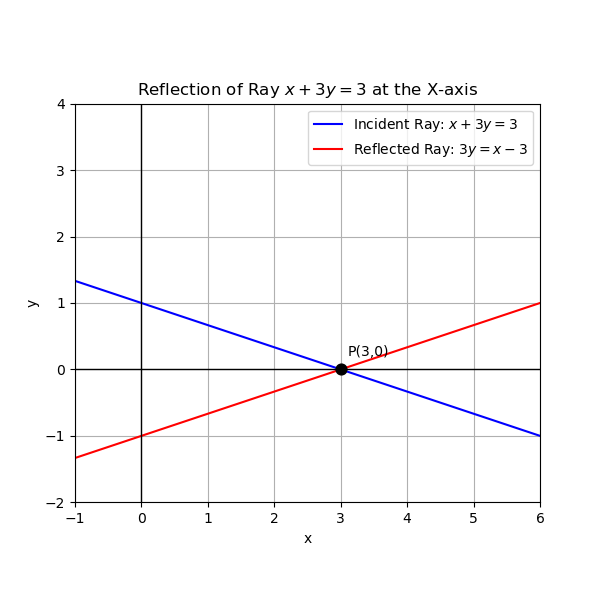
\includegraphics[width=0.6\columnwidth]{Figs/Fig1.png}
\end{center}
\caption{}
\label{fig:Fig.1}
\end{figure}

\end{document}
